\documentclass[journal]{IEEEtran}
\usepackage[spanish]{babel}
\usepackage[utf8]{inputenc}
\usepackage{enumerate}
\usepackage{graphicx}
\usepackage{booktabs}
\usepackage{physics}

\hyphenation{op-tical net-works semi-conduc-tor}


\begin{document}
\title{Reporte de Práctica: Movimiento Circular }

\author{Licenciatura en Física	\\
Universidad Nacional Autónoma de México - Facultad de Ciencias\\
Profesor: José Alfredo Morales Pérez\\
Ayud. Lab.	Miranda García Ávila\\
Integrantes: Jeshua Roberto Estrada Ocampo,~\IEEEmembership{424003085}\\

            
\thanks{}% <-this % stops a space
\thanks{}% <-this % stops a space
\thanks{}}

\markboth{Laboratorio de Mecánica}%
{Shell \MakeLowercase{\textit{et al.}}: Bare Demo of IEEEtran.cls for Journals}

\maketitle

\begin{abstract}
-En esta práctica de laboratorio se estudió el movimiento circular uniforme (MCU) mediante la observación de un objeto que se desplaza a lo largo de una trayectoria circular con velocidad constante. Se utilizó un dispositivo de rotación controlada para mantener una velocidad angular constante y medir las fuerzas centrípetas actuantes. Se determinaron las relaciones entre las variables involucradas y se verificaron las leyes teóricas que describen el MCU. Los resultados obtenidos fueron consistentes con las predicciones teóricas, validando así los principios del movimiento circular uniforme.
\end{abstract}

\begin{IEEEkeywords}
Movimiento circular uniforme, velocidad angular, fuerza centrípeta, trayectoria circular, cinemática.
\end{IEEEkeywords}

\IEEEpeerreviewmaketitle

\section{INTRODUCCIÓN}
\subsection{Planteamiento}

\IEEEPARstart  {E}l estudio del movimiento circular uniforme (MCU) es fundamental en la mecánica clásica, ya que permite comprender cómo los objetos se comportan cuando se mueven en trayectorias circulares con velocidad constante. Este tipo de movimiento se encuentra en diversas aplicaciones prácticas, desde el funcionamiento de motores y maquinaria hasta fenómenos astronómicos como la órbita de los planetas. La práctica de laboratorio se justifica porque ofrece la oportunidad de observar y medir directamente las fuerzas y aceleraciones involucradas en el MCU, proporcionando una experiencia tangible y práctica que complementa la teoría aprendida en clase. Además, el análisis experimental del MCU ayuda a reforzar conceptos clave de la física, como la fuerza centrípeta y la relación entre velocidad angular, radio y período.\\

\subsubsection{Objetivos Generales}

 - Poder comparobar que en un cuerpo que se mueve con trayectoria circular bajo acción de la gravedad es en realidad un m.c.u, (movimiento circular uniforme).\\

\subsubsection{Objetivos particulares}
- Medir la velocidad angular y el período de un objeto en movimiento circular uniforme.
- Evaluar la precisión de las mediciones experimentales y compararlas con las predicciones teóricas.
- Identificar y discutir las posibles fuentes de error en el experimento.
\subsubsection{Hipótesis}
Si un objeto se mueve en una trayectoria circular con velocidad constante, entonces la fuerza centrípeta que actúa sobre el objeto será directamente proporcional al cuadrado de su velocidad angular y al radio de la trayectoria. Esta relación se puede verificar midiendo la fuerza centrípeta y comparándola con los valores teóricos calculados.
\\


\section{MARCO TEÓRICO}
En el MCU, un objeto se mueve en una trayectoria circular con un radio r constante y una velocidad angular \(\omega\) constante. La velocidad angular \(\omega\) se define como el ángulo barrido por unidad de tiempo, y se mide en radianes por segundo (rad/s).
La fuerza centrípeta es la fuerza neta que actúa sobre un objeto en MCU, dirigiéndolo hacia el centro de la trayectoria circular. Según la segunda ley de Newton, esta fuerza es igual al producto de la masa 
m del objeto y su aceleración centrípeta:

\begin{equation}\label{eq:2}
 \omega = \frac{\Delta\vartheta}{\Delta t}
\end{equation}

donde \(\Delta\vartheta\) es el ángulo barrido en radianes
\(\Delta t\) es el intervalo de tiempo.\\
y la dirección del movimiento. Cuando la fuerza se aplica en la misma dirección que el movimiento (\(\vartheta = 0\) ) la fórmula se simplifica a:

\begin{equation}\label{eq:1}
 F_c = ma_c = m\frac{\omega^2}{r} = m\omega^2r
\end{equation}

donde v es la velocidad lineal y r es el radio de la trayectoria circular

Período y Frecuencia
El período T es el tiempo que tarda un objeto en completar una vuelta completa en la trayectoria circular. La frecuencia f es el número de vueltas completadas por unidad de tiempo. La relación entre el período y la frecuencia es:

\begin{equation}\label{eq:2}
 T = \frac{1}{f}
\end{equation}
 
Además, la velocidad angular \(\omega\) está relacionada con el período y la frecuencia mediante las siguientes formulas

\begin{equation}\label{eq:4}
\omega = 2\pi f = \frac{2\pi}{T}
\end{equation}

\section{ MATERIALES}
\begin{itemize}
\item Disco giratorio con soporte \item hilo \item plastilina \item una pesa
\item cinta adhesiva 

\end{itemize}

\section{DESARROLLO EXPERIMENTAL}
\begin{figure}[h]
    \centering
    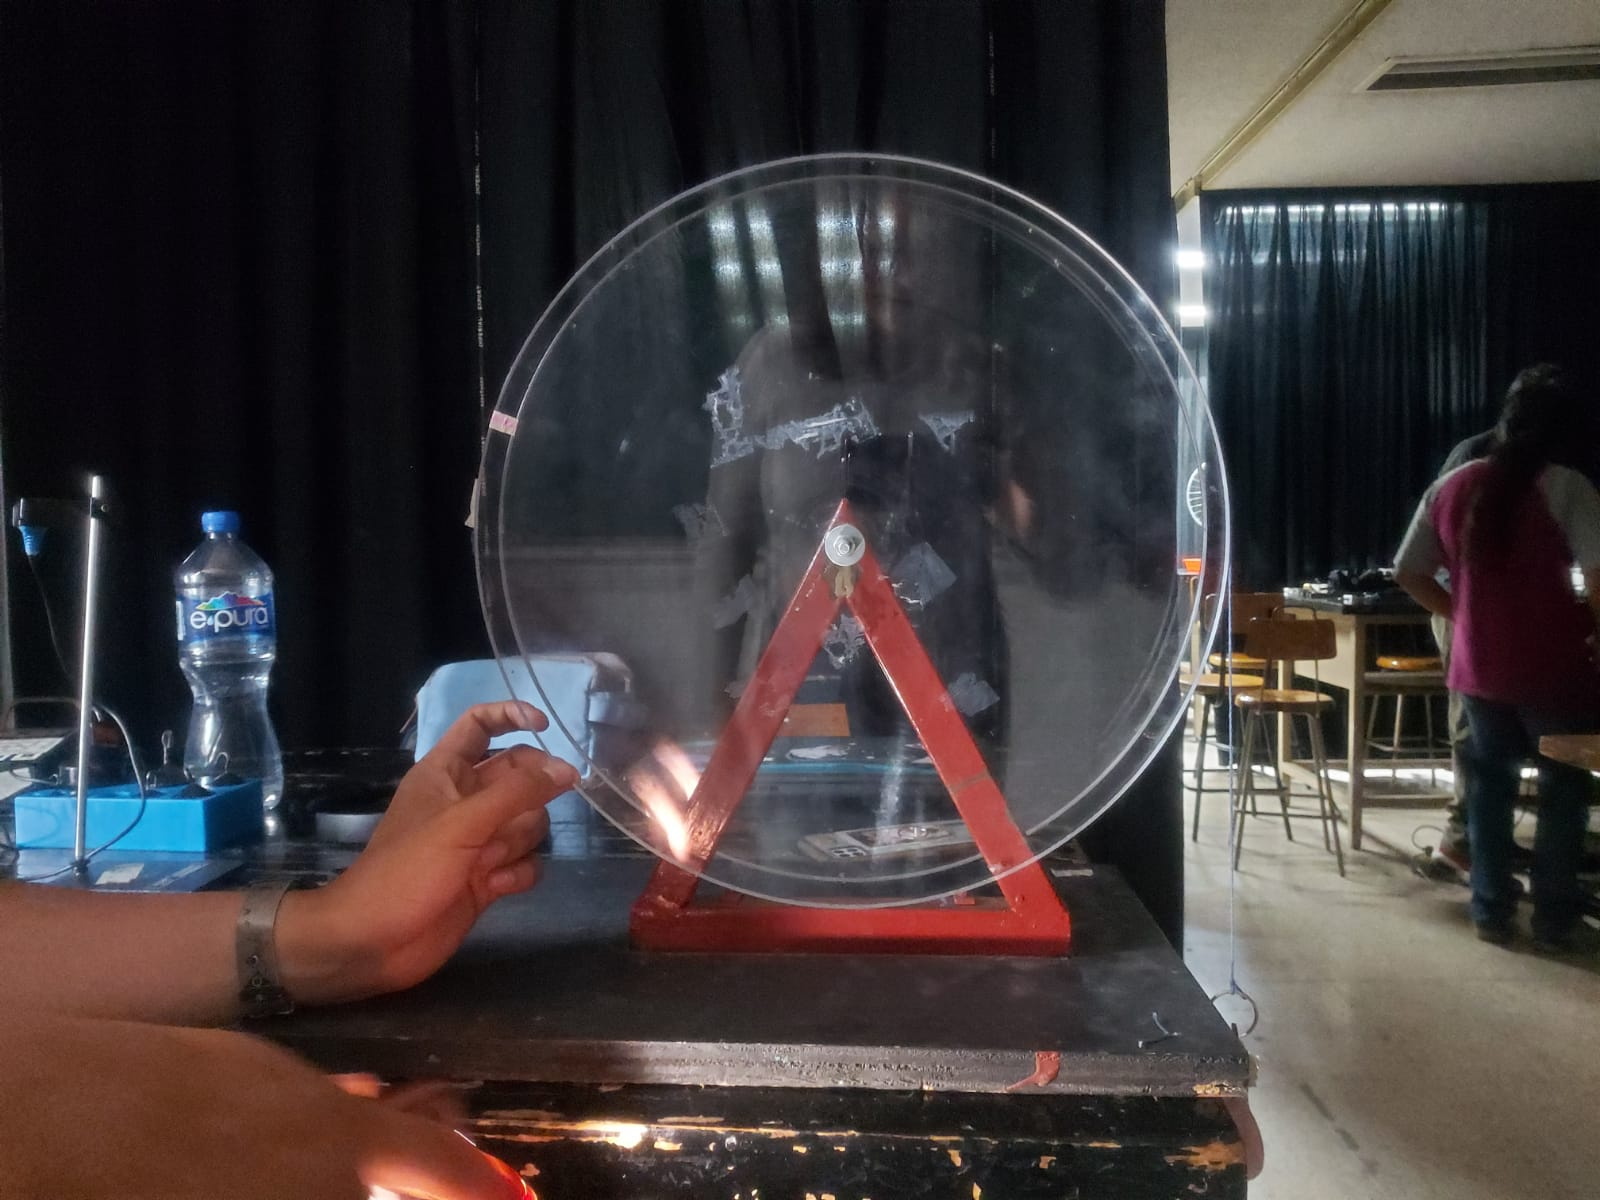
\includegraphics[width=1\linewidth]{disc.png}
    \caption{Proceso del montaje del movimiento circular}
    \label{fig:enter-label}
\end{figure}\\
Para obtener resultados precisos y confiables en el estudio del movimiento circular uniforme (MCU), es esencial establecer condiciones ideales que minimicen los errores experimentales. Las siguientes condiciones deben ser consideradas:

Superficie Estable y Nivelada: El equipo debe estar colocado sobre una superficie plana y nivelada para evitar inclinaciones que puedan afectar el movimiento del disco.
Ausencia de Vibraciones: La mesa y el entorno deben estar libres de vibraciones que puedan introducir fluctuaciones en el movimiento del disco.

Montaje del Disco Giratorio:

Coloque el disco giratorio al borde de una mesa estable y nivelada. Asegúrese de que el disco permanezca fijo y no se tambalee. Esto se puede lograr utilizando soportes o abrazaderas para asegurar el disco firmemente a la mesa.

Preparación del Sistema de Pesas y Hilo:

Ate una pesa al extremo de un hilo resistente. El otro extremo del hilo debe ser enrollado cuidadosamente alrededor del perímetro de la circunferencia del disco.
Asegúrese de que el hilo esté bien sujeto y que no haya nudos o torsiones que puedan interferir con su desenrollado suave.

Generación de Energía Cinética:

Levante la pesa para darle una cierta altura. Esto otorga al sistema energía potencial gravitatoria.
Libere la pesa de manera que la energía potencial se convierta en energía cinética, lo que hará que el disco comience a girar. Asegúrese de que el movimiento sea suave y sin interrupciones.

Simulación de la Partícula en Movimiento:

Pegue un trozo de cinta adhesiva en el borde del disco. Esta cinta servirá para simular una partícula en movimiento en la periferia del disco.
La cinta debe estar bien adherida y no debe agregar un peso significativo que altere el balance del disco.
\hfill 

\section{RESULTADOS}

En esta sección se presenta la gráfica realizada con las tablas de datos correspondientes al cálculo de las velocidades angulares ($\omega$) en cada caso de movimiento circular uniforme. Estos datos se obtuvieron utilizando el software Tracker, que permite describir las trayectorias de los cuerpos en movimiento.\\

Nota: De las seis repeticiones realizadas, se descartaron dos debido a que no proporcionaban información adecuada para la descripción del movimiento. Esto se debió a que los tiempos de duración de los movimientos en los videos correspondientes eran muy cortos, y el disco no lograba completar un número suficiente de vueltas para describir una velocidad constante.\\

Nota 2: Finalmente, se consideró solo una repetición, ya que realizar las demás valoraciones resultaría muy complicado. Las dificultades encontradas en la caracterización y obtención de resultados llevaron a la conclusión de que el método utilizado para tomar los datos no era el más adecuado para medir la velocidad angular. Esto se debió a un error sistemático en el uso del software para la descripción del movimiento, específicamente en la medición de ángulos respecto al tiempo. Por lo tanto, se hizo una aproximación de los resultados utilizando únicamente las gráficas que se pudieron obtener.\\

\begin{figure}[h]
    \centering
    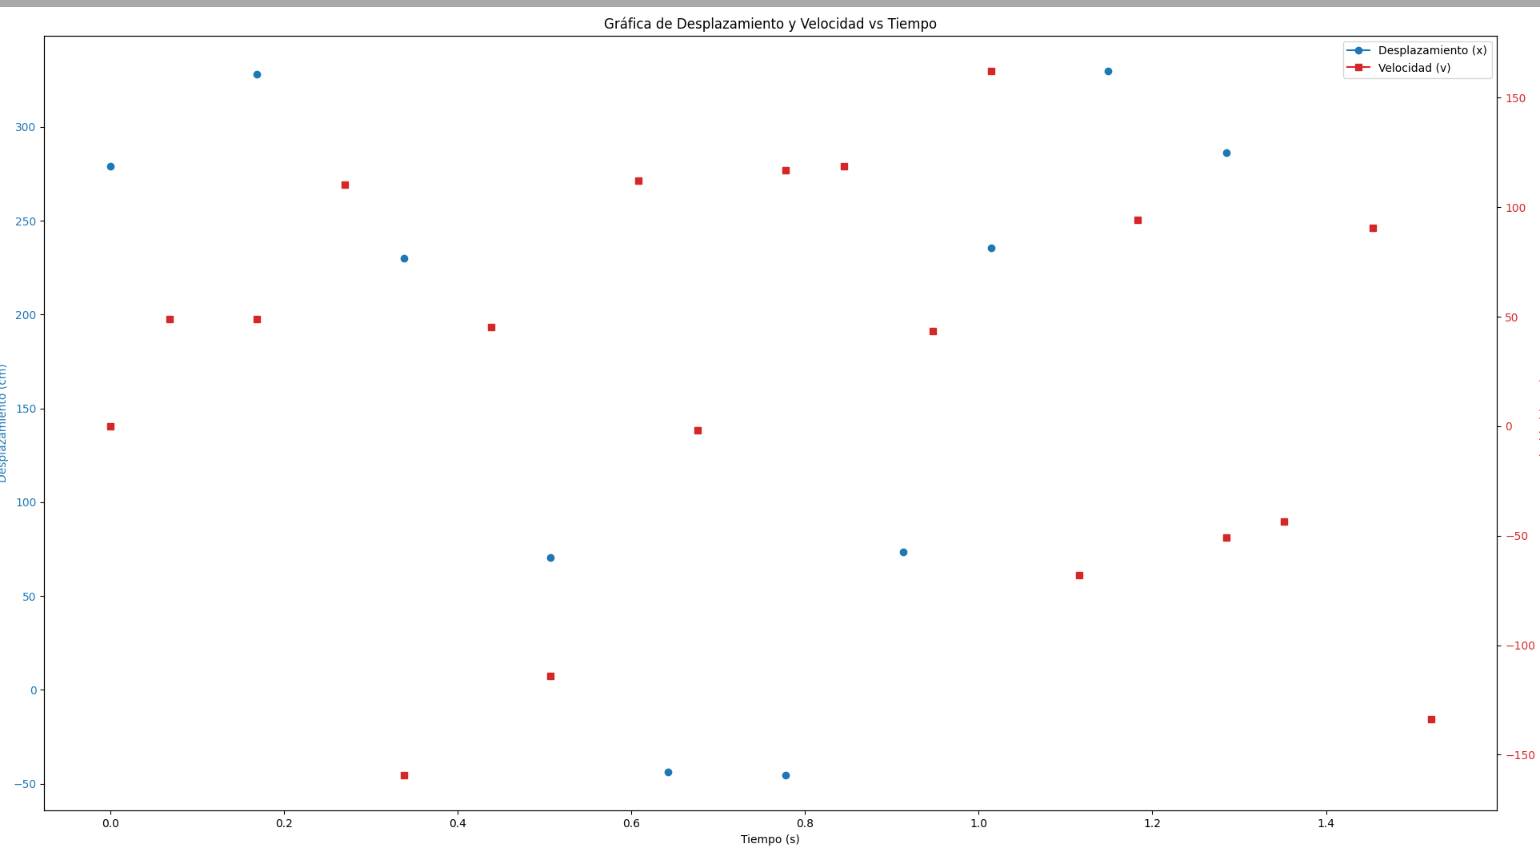
\includegraphics[width=1\linewidth]{datos.png}
    \caption{Gráfica sinusoidal del MCU con puntos disconexos}
    \label{fig:enter-label}
\end{figure}\\
\newpage
\begin{figure}[h]
    \centering
    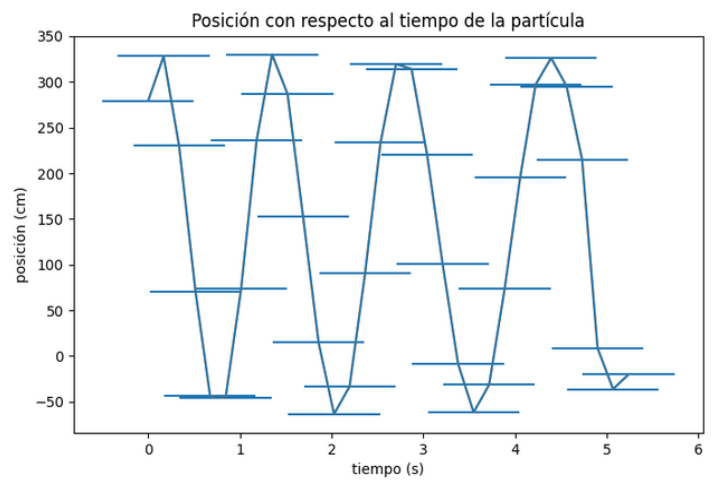
\includegraphics[width=1\linewidth]{conexidad1.png}
    \caption{Posición con respecto al tiempo conexa}
    \label{fig:enter-label}
\end{figure}\\
\textit{ }\\
\begin{figure}[h]
    \centering
    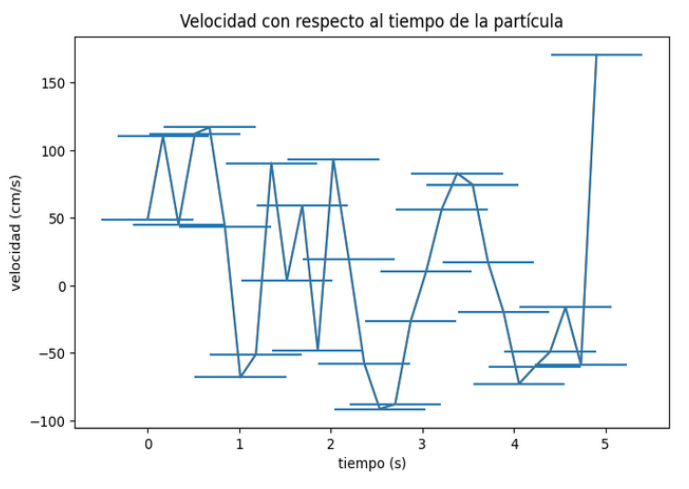
\includegraphics[width=1\linewidth]{conexidad2.png}
    \caption{Velocidad con respecto al tiempo conexa}
    \label{fig:enter-label}
\end{figure}

\section{DISCUSIÓN}
En esta sección se presentan las gráficas correspondientes a la tabla anterior, las cuales están limitadas únicamente a la primera medición debido a las dificultades mencionadas anteriormente en el manejo de los datos y del software utilizado para describir el movimiento.\\

Gráfica 1: Esta gráfica representa la posición de la partícula inmersa en un sistema de movimiento circular uniforme (MCU). Fue lo único que se pudo describir correctamente en este análisis, ya que se ajusta a la ecuación (3) del marco teórico. Se observa claramente la trayectoria sinusoidal, característica del movimiento circular, que se manifiesta a través de un sistema cartesiano no giratorio. Este movimiento periódico está en concordancia con lo señalado en el marco teórico. Es importante mencionar que las barras de error se programaron para ambos ejes, aunque los valores de posición no correspondieron a los reales debido a un fallo del programa. Por lo tanto, no se respetó la incertidumbre de 0.5 en las tablas de datos y no se reflejan en el gráfico.\\

Gráfica 2: Esta gráfica muestra la velocidad de verificación de la tabla o cuadro 1. Se esperaba que representara una línea recta, pero debido al carácter oscilatorio en la posición, se obtuvieron valores negativos para algunos valores de $x$. Se buscaba medir el módulo de esta velocidad, pero debido a la falta de habilidad para obtener datos durante el experimento, la gráfica no refleja el comportamiento esperado.\\

Se descartaron las demás repeticiones precisamente porque se esperaba que se presentara la misma situación errónea, lo que impedía obtener resultados significativos. Por lo tanto, se presentan los resultados de una sola repetición para exponer esta situación en su totalidad.

\section{ CONCLUSIONES} 
De acuerdo con los objetivos planteados al inicio, se logró lo siguiente:\\

Se consiguió generar un movimiento circular uniforme (MCU), como se evidencia en la primera gráfica que muestra el comportamiento general del sistema. Sin embargo, no se logró medir el módulo de la velocidad angular para comprobar que todos los módulos en este movimiento fueran iguales.\\

Debe resaltarse que se descartaron cinco medidas debido a que los datos fueron significativamente afectados por un mal manejo del software de análisis de video, lo cual se considera un error sistemático cometido tanto por el operador de los datos como por el software. Además, la técnica utilizada para la obtención de velocidades fue inadecuada. Por lo tanto, al no poder obtener datos confiables con las medidas disponibles, se decidió descartarlas.\\

Se sugiere que en futuros experimentos que involucren la obtención de la velocidad angular, se recomienda utilizar fotocompuertas para recolectar los datos de manera más eficiente y evitar problemas relacionados con cambios de signo debido al sistema de referencia utilizado. Esto permitirá una medición más precisa y confiable del módulo de la velocidad angular.\\


% you can choose not to have a title for an appendix
% if you want by leaving the argument blank
\section{ REFERENCIAS}
\begin{itemize}
\item Serway, R. A., Jewett, J. W. (2008). "Física para ciencias e ingeniería.".
\item Resnick-Halliday. "Física Vol. 2, 5$^{ta}$ Edición, Editorial CECSA, México, 2005".
\item Aranzeta, C. G. (1986). "Introducción a la metodología experimental."
\item Oda-Noda, B. (2005). "Introducción al análisis gráfico de datos experimentales." 
\end{itemize}
% use section* for acknowledgment







\end{document}